\section{Security}
\label{sec:security}

The trust model of NLSR is semi-hierarchical. An example certificate signing hierarchy is show in Figure~\ref{fig:trust}.
In this hierarchy, each entity's name and corresponding certificate name follow the convention described in Table~\ref{table:kname}.

\begin{figure}
\centering
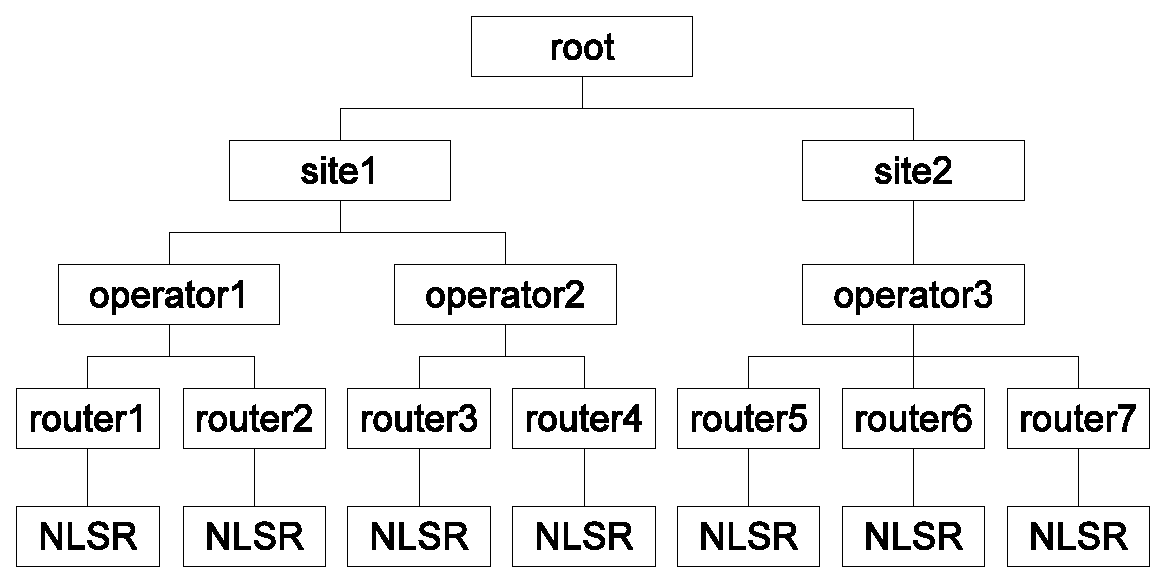
\includegraphics[width=0.5\linewidth]{figures/trust-hierarchy.eps}
\caption{NLSR Trust Hierarchy}
\label{fig:trust}
%\vspace{-3mm}
\end{figure}

\begin{table}
\centering	
	\caption{Key Names}
	\small
	\begin{tabular}{|l|l|}
	\hline
	\bfseries {Key Owner} & \bfseries {Key Name}\\ \hline
	Network & /$<$network$>$/KEY/$<$key$>$\\ \hline
	Site & /$<$network$>$/$<$site$>$/KEY/$<$key$>$\\ \hline
	Operator & /$<$network$>$/$<$site$>$/$<$operator$>$/KEY/$<$key$>$\\\hline
	Router & /$<$network$>$/$<$site$>$/$<$router$>$/KEY/$<$key$>$\\\hline
	NLSR & /$<$network$>$/$<$site$>$/$<$router$>$/NLSR/KEY/$<$key$>$\\\hline
	\end{tabular}
	\label{table:kname}
	\vspace{-3mm}
\end{table}

\subsection{Creating Keys and Certificates}

The process to create keys and certificates for this hierarchy can be performed using the \texttt{ndnsec}~\cite{ndnsec} tools included with \texttt{ndn-cxx}~\cite{NDNCXX}.
The steps to create the keys and certificates is outlined below:

\begin{enumerate}
\item Create keys for Root: \\ \texttt{ndnsec-keygen \$ROOT\_NAME > \$ROOT\_KEY\_OUTPUT\_FILE}
\item Create certificate for Root: \\ \texttt{ndnsec-certgen -N \$ROOT\_NAME -p \$ROOT\_NAME \$ROOT\_KEY\_OUTPUT\_FILE > \$ROOT\_CERT\_OUTPUT\_FILE}
\item For each site, create keys and certificates:
  \begin{enumerate}
  \item On the Site machine, generate keys for the Site: \\ \texttt{ndnsec-keygen \$SITE\_NAME > \$SITE\_KEY\_OUTPUT\_FILE}
  \item Copy \texttt{\$SITE\_KEY\_OUTPUT\_FILE} over to the machine where the Root certificate was created.
  \item Generate a certificate for the Site on the Root machine: \\ \texttt{ndnsec-certgen -N \$SITE\_NAME -p \$SITE\_NAME -s \$ROOT\_NAME \$SITE\_KEY\_OUTPUT\_FILE > \$SITE\_CERT\_OUTPUT\_FILE}
  \item Copy \texttt{\$SITE\_CERT\_OUTPUT\_FILE} over to the Site machine.
  \item Install the certificate on the Site machine: \\ \texttt{ndnsec-cert-install -f \$SITE\_CERT\_OUTPUT\_FILE}
  \item On the Site machine, create the Operator keys: \\ \texttt{ndnsec-keygen \$OP\_NAME > \$OP\_KEY\_OUTPUT\_FILE}
  \item On the Site machine, create the Operator certificate: \\ \texttt{ndnsec-certgen -N \$OP\_NAME -p \$OP\_NAME -s \$SITE\_NAME \$OP\_KEY\_OUTPUT\_FILE > \$OP\_CERT\_OUTPUT\_FILE}
  \item On the Site machine, create the Router keys: \\ \texttt{ndnsec-keygen \$ROUTER\_NAME > \$ROUTER\_KEY\_OUTPUT\_FILE}
  \item On the Site machine, create the Router certificate: \\ \begin{small}\texttt{ndnsec-certgen -N \$ROUTER\_NAME -p \$ROUTER\_NAME -s \$OP\_NAME \$ROUTER\_KEY\_OUTPUT\_FILE > \$ROUTER\_CERT\_OUTPUT\_FILE}\end{small}
  \end{enumerate}
  \item When NLSR starts, it will automatically create the NLSR keys and certificates for the router.
\end{enumerate}

\subsection{Certificate Publishing}

In a network, every router must have the root certificate configured as a trust anchor for the \texttt{validator} in the configuration file. If two routers in a network do not share a common trust anchor, then when one seeks to validate the data of the other, they may be unable to establish trust in their signature. This is, of course, because of how the trust hierarchy is set up: you trust the person that signed some router's certificate, because it was signed by the site certificate, and the site certificate was signed by the region, etc., and the $nth$ certificate was signed by the root certificate, which is your trust anchor, so you ``just trust it''. Moreover, if your trust anchor is \emph{before} their trust anchor in the ``chain'', then they will be able to trust you, but you will not be able to trust them.

For each site, at least one router should publish the site certificate, and at least one router should publish the certificate of the site operator.
Each router should publish its own certificate. This is a matter of performance; a network would work if all certificates for all nodes were kept centrally, but distributing the certificates in this way improves performance.
All this information must be explicitly specified in the configuration file.

For example, the following configuration file indicates that NLSR should publish the site certificate and the router certificate:

\begin{verbatim}
...
security
{
  validator
  {
    ...
  }
  cert-to-publish "$SITE_CERT_OUTPUT_FILE"   ; name of the site certificate file
  cert-to-publish "$SITE_CERT_OUTPUT_FILE"   ; name of the router certificate file
  ...
}
\end{verbatim}
